\documentclass[10pt,pdftex]{article}
\usepackage{graphicx}
\usepackage{natbib}
\bibliographystyle{apalike}
\usepackage{caption}
\renewcommand{\captionfont}{\fontsize{9pt}{10pt}\selectfont}
\renewcommand{\thefigure}{S\arabic{figure}}
\renewcommand{\thetable}{S\arabic{table}}

\addtolength{\textwidth}{3cm}\addtolength{\hoffset}{-1.5cm}\addtolength{\textheight}{4cm}\addtolength{\voffset}{-2cm}

\title{Aligning sequence reads, clone sequences and assembly contigs with BWA-MEM (Supplementary Information)}
\author{Heng Li}
\date{}

\begin{document}

\maketitle

\section{Workflow of BWA-MEM}

\begin{figure}[!htb]
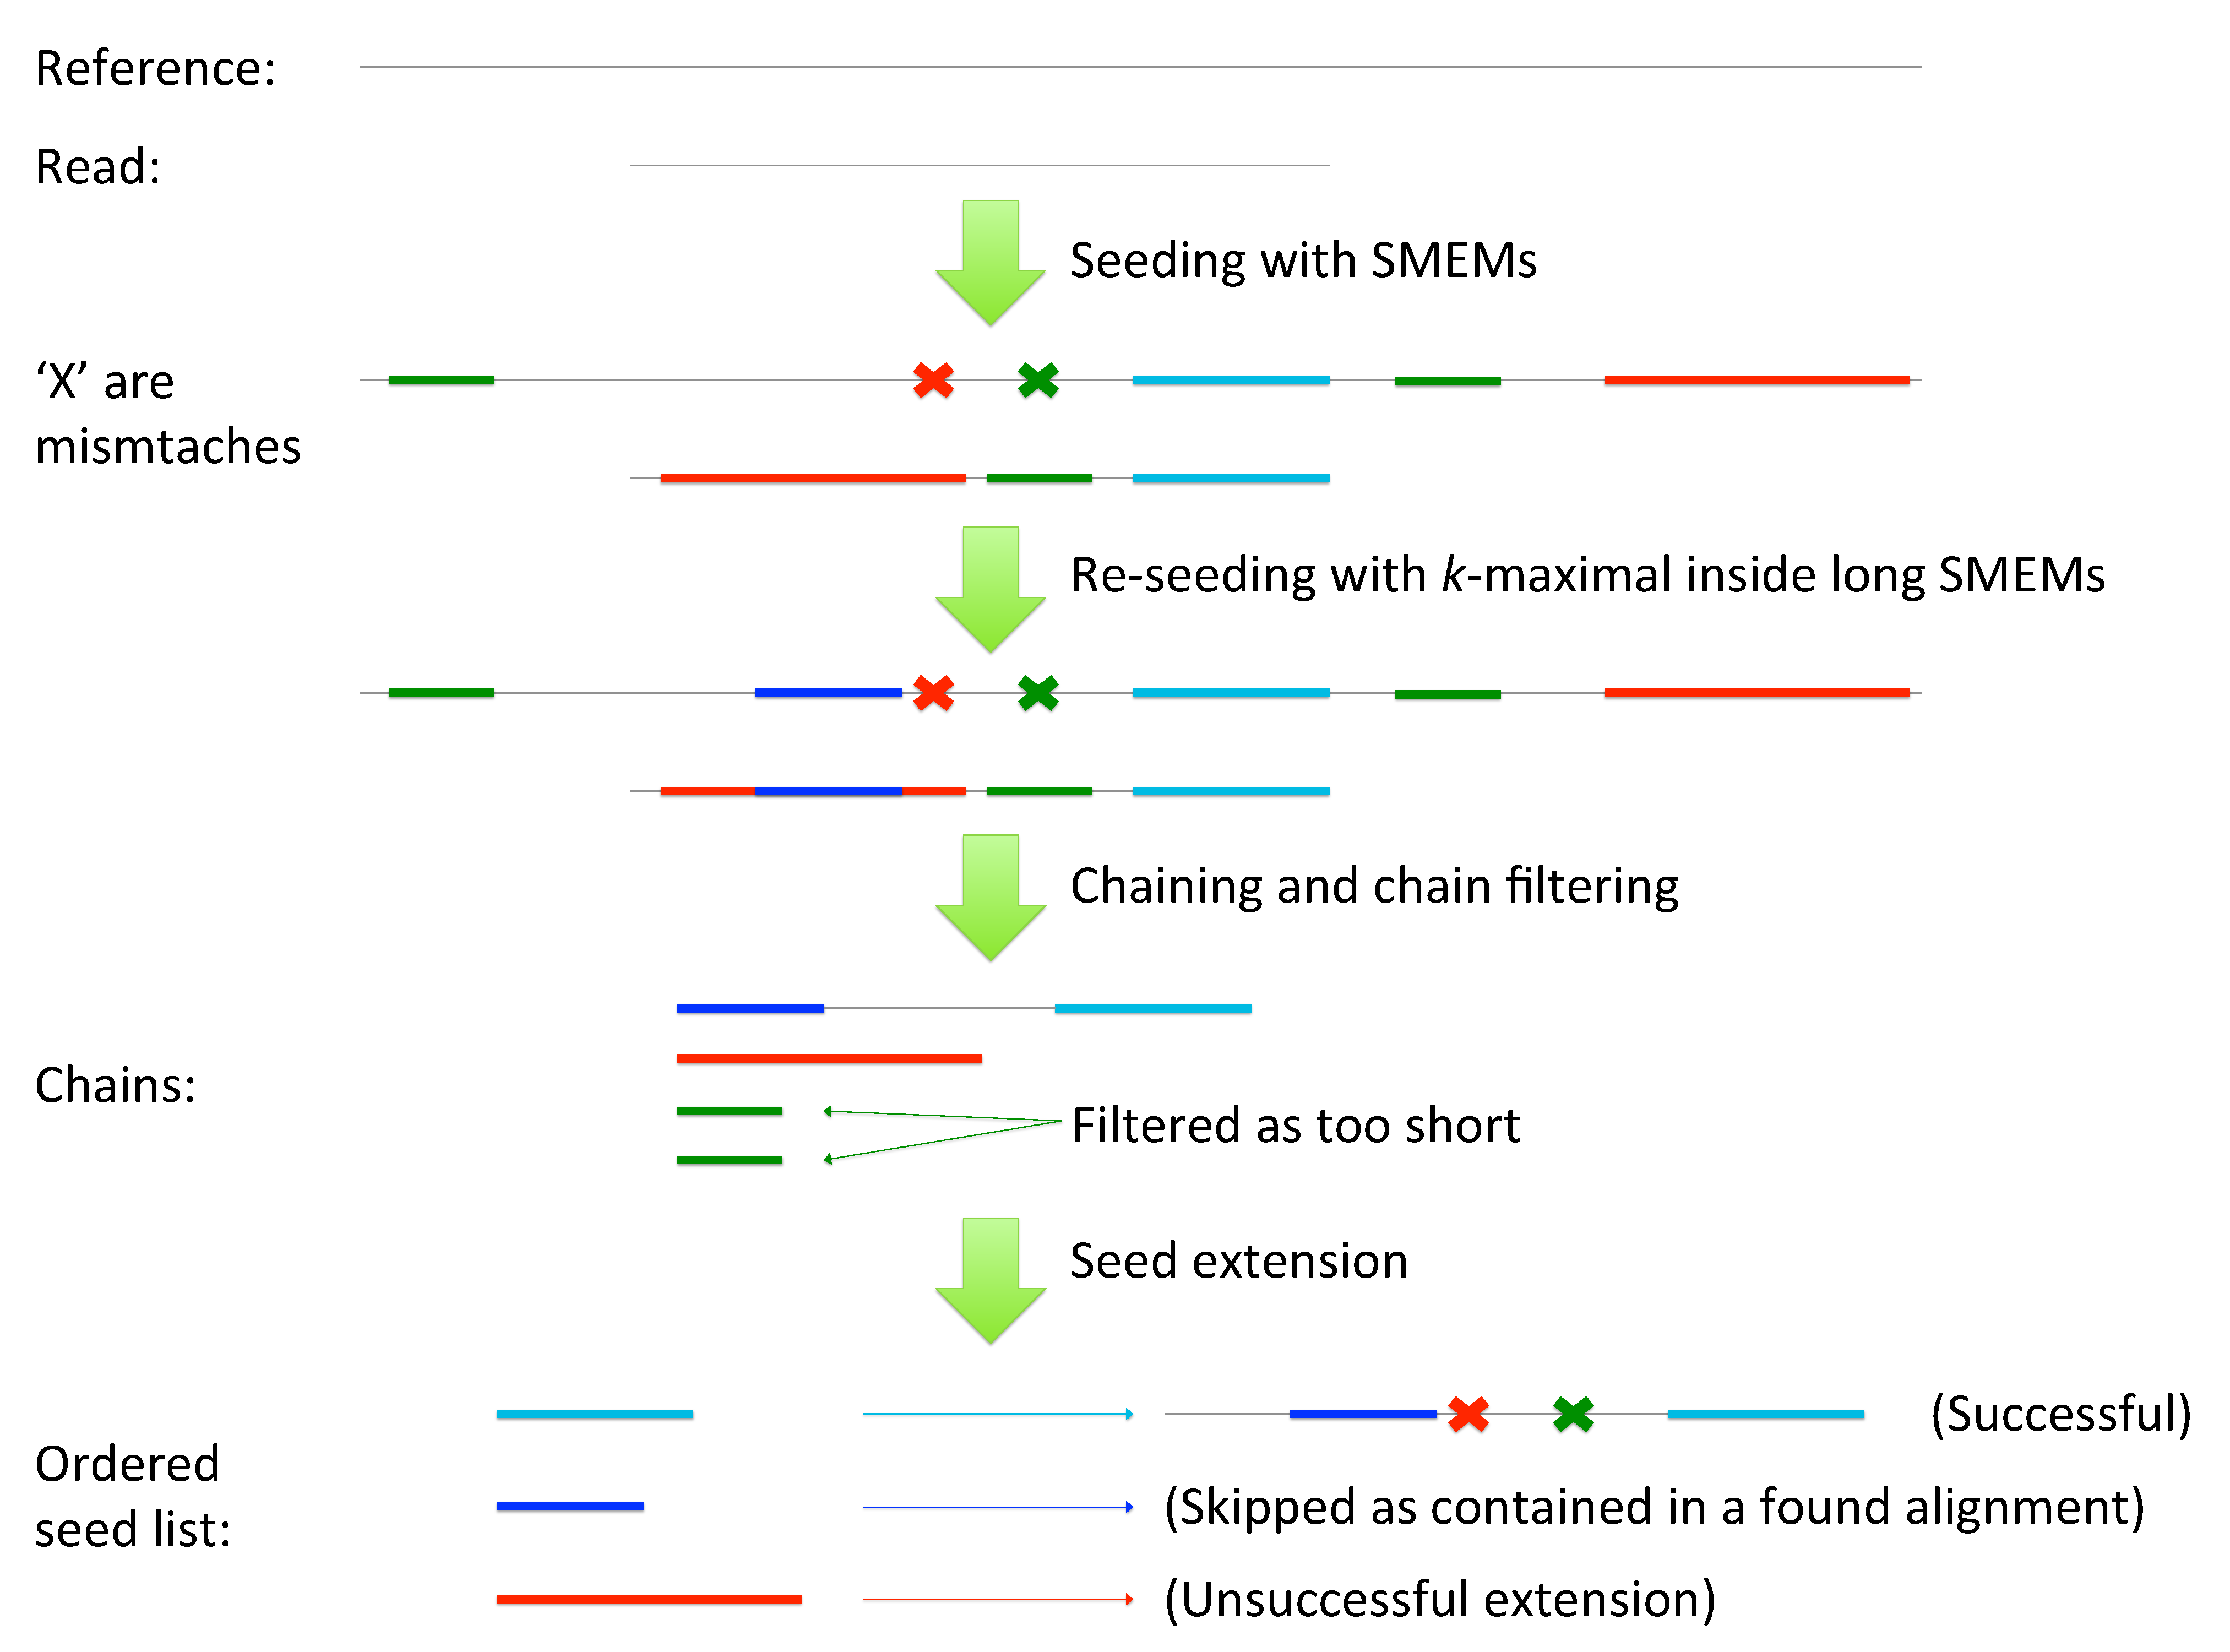
\includegraphics[width=\textwidth]{mem-flow}
\caption{BWA-MEM workflow.}
\end{figure}

\section{Evaluation on bacterial genome alignment}
To evaluate the performance for even longer query sequences, we aligned the
{\it E. coli} K-12 MG1655 substrain (AC:NC\_000913; 4.6Mb in length) against
the 536 strain (AC:NC\_008253) with both BWA-MEM and
nucmer~\citep{Kurtz:2004zr}. Nucmer finished the alignment in 25 seconds,
giving 105,505 substitution differences between the strains. BWA-MEM is slower.
It finished the alignment in 131 seconds, reporting 104,321 substitutions of
which 102,241 overlapping with the nucmer output. Manual examination of the
substitutions unique to each aligner reveals that most of them fall in short
regions with very high divergence. It is unclear which aligner is better. Note
that although nucmer is faster in the evaluation, only BWA-MEM scales well to
large genomes.

\section{Evaluation of additional mappers}
In addition to the mappers shown in the main text, we have also evaluated
SeqAlto~\citep{Mu:2012fk}, GSNAP~\citep{Wu:2010uq}, STAR~\citep{Dobin:2013kx},
SMALT (http://bit.ly/smalt-aln) and LAST~\citep{Shrestha:2013aa}. The detailed
command lines are shown in Table S1, S2 and S3.

\begin{table}[!tbhp]
\footnotesize
\centering
\begin{tabular}{lll}
\hline
Program & Version & Indexing command line \\
\hline
Bowtie2 & 2.1.0 & bowtie2-build ref.fa ref.bt2 \\
BWA & 0.7.0 & bwa index ref.fa (version 0.6.2 for BWA and BWA-SW)\\
Cushaw2 & 2.1.8 & cushaw2\_index -a bwtsw ref.fa \\
GEM & 2012-10-28 & gem-indexer -i ref.fa -o ref \\
GSNAP & 2013-03-31 & gmap\_build -d ref.gmap ref.fa \\
LAST & 278 & lastdb -m1111110 ref.last ref.fa \\
Novoalign & 2.08.03 & novoindex -s3 ref.novo ref.fa \\
SeqAlto & 0.5-r123 & seqalto index ref.fa 22 ref.alto \\
SMALT & 0.7.2 & smalt index -k20 -s3 ref.smalt ref.fa \\
STAR & 2.3.0e & STAR --runMode genomeGenerate --genomeDir star --genomeFastaFiles ref.fa \\
\hline
\end{tabular}
\caption{Program versions and indexing command lines}
\end{table}

\begin{table}[!tbhp]
\footnotesize
\centering
\begin{tabular}{lrrp{9cm}}
\hline
Algorithm & Time:s & Mem:GB & Command line \\
\hline
Bowtie2   & 582 & 3.1 & bowtie2 -x ref.bt2 r12.fq \\
BWA       & 1055& 4.5 & bwa aln -f r12.sai ref.fa r12.fq; bwa samse ref.fa r12.sai r12.fq \\
BWA-SW    & 1002& 5.1 & bwa bwasw ref.fa r12.fq \\
BWA-MEM   & 467 & 5.1 & bwa mem ref.fa r12.fq \\
Cushaw2   & 967 & 3.3 & cushaw2 -r ref.fa -q r12.fq \\
GEM       & 426 & 4.0 & gem-mapper -I ref.gem -i r12.fq -e5 -m5 -s1 \\
GSNAP     & 5553& 5.0 & gsnap -Asam -d ref.gmap r12.fq \\
LAST      & 4302& & lastal -Q1 ref.last r12.fq $|$ last-map-probs.py -m 0.5 - $|$ maf-convert.py sam - \\
Novoalign & 3960& 6.0 & novoalign -oSAM -rRandom -d ref.novo -f r12.fq \\
SeqAlto   & 850 & 6.8 & seqalto align ref.alto -1 r12.fq \\
SMALT     & 3859& 3.4 & smalt map -f samsoft ref.smalt r12.fq \\
STAR      & $<$128 & 26.6& STAR --genomeDir star --readFilesIn r12.fq --runThreadN 1 --outFilterMultimapNmax 1 --chimSegmentMin 30 --genomeLoad LoadAndKeep \\
\hline
\end{tabular}
\caption{CPU time in seconds, peak memory in GB and command lines for
single-end mapping.  Programs were run on a single Xeon CPU core clocked at
3.47GHz with 96GB RAM. They were timed for the second run to minimize index
loading time as the system can usually cache the index in memory. However, STAR
still spent significant amount of time for loading the index. The actual CPU
time spent on alignment should be shorter.}
\end{table}

\begin{table}[!tbhp]
\footnotesize
\centering
\begin{tabular}{lrrp{9cm}}
\hline
Algorithm & Time:s & Mem:GB & Command line \\
\hline
Bowtie2   & 545& 3.1& bowtie2 -x ref.bt2 -1 r1.fq -2 r2.fq -X650 \\
BWA       & 1055& 5.1 & bwa aln -f r1.sai ref.fa r1.fq; bwa -f r2.sai ref.fa r2.fq; bwa sampe ref.fa r1.sai r2.sai r1.fq r2.fq \\
BWA-SW    & 1002& 5.1 & bwa bwasw ref.fa r1.fq r2.fq \\
BWA-MEM   & 467 & 5.1 & bwa mem ref.fa r1.fq r2.fq \\
Cushaw2   & 1026& 3.3 & cushaw2 -r ref.fa -q r1.fq r2.fq \\
GEM       & 529 & 4.0 & gem-mapper -I ref.gem -1 r1.fq -2 r2.fq -e5 -m5 -s1 -pb \\
GSNAP     & 3514& 5.0 & gsnap -Asam -d ref.gmap r1.fq r2.fq \\
LAST      & 5386& & lastal -Q1 ref.last r1.fq $>$ r1.maf; lastal -Q1 ref.last r2.fq $>$ r2.maf; last-pair-probs.py -m 0.5 r1.maf r2.maf $|$ maf-convert.py sam - \\
Novoalign & 2585& 6.0 & novoalign -i 500 50 -oSAM -rRandom -d ref.novo -f r1.fq r2.fq \\
SeqAlto   & 879 & 6.8 & seqalto align ref.alto -1 r1.fq -2 r2.fq -i 650 -m 500 \\
SMALT     & 1705& 3.4 & smalt map -f samsoft -i 650 -j 450 ref.smalt r1.fq r2.fq \\
STAR      & $<$135& 26.6& STAR --genomeDir star --readFilesIn r1.fq r2.fq --runThreadN 1 --outFilterMultimapNmax 1 --chimSegmentMin 30 --genomeLoad LoadAndKeep \\
\hline
\end{tabular}
\caption{CPU time in seconds, peak memory in GB and command lines for mapping paired-end reads.}
\end{table}

\begin{figure}
\centering
\includegraphics[width=\textwidth]{alnroc-color-se}\\
\includegraphics[width=\textwidth]{alnroc-color-pe}
\caption{Percent mapped reads as a function of the false alignment rate under
different mapping quality cutoff. STAR does not output mapping quality. Almost
all GSNAP alignments have mapping quality 18. Their accuracy is represented by
a single dot only.}
\end{figure}

\pagebreak
\bibliography{bwamem}

\end{document}
